% -------------------- Packages --------------------
%  Document Class --------------------
\documentclass[12pt,a4paper]{report}
 
% -------------------- Language and Encoding --------------------
\usepackage[utf8]{inputenc}    % Input encoding
\usepackage[T1]{fontenc}       % Font encoding
\usepackage[english]{babel}    % Language

%  Typography and Fonts --------------------
\usepackage{lmodern}           % Improved font rendering

%  Page Layout --------------------
\usepackage[a4paper, margin=1in]{geometry}  % Page size and margins

%  Colors and Graphics --------------------
\usepackage{xcolor}            % Custom colors
\usepackage{graphicx}          % For including images
\usepackage{caption}

%  PDF and External Docs --------------------
\usepackage{pdfpages}          % Insert external PDFs
\usepackage{afterpage}         % Delayed page commands

%  Title and Section Formatting --------------------
\usepackage{titlesec}          % Custom section formatting
\usepackage{titling}           % Advanced title control

%  Hyperlinks --------------------
% \usepackage[hidelinks]{hyperref} % Clickable links without colored boxes
\usepackage[draft]{hyperref} % Clickable links without colored boxes

%  Spacing and Paragraphs --------------------
\usepackage{setspace}          % Optional: control line spacing
\usepackage{indentfirst}       % Indent first paragraph after section
\setlength{\parindent}{15pt}   % Paragraph indentation
\setlength{\parskip}{0.7em}    % Space between paragraphs

%  Figures --------------------
\usepackage{chngcntr}
\usepackage{float} % provides the H placement specifier
\counterwithin{figure}{chapter}

%  Section Numbering and Depth --------------------
% \renewcommand{\thesection}{\Roman{section}}
% \renewcommand{\thesubsection}{\thesection.\arabic{subsection}}
% \renewcommand{\thesubsubsection}{\thesubsection.\alph{subsubsection}}

\renewcommand\thechapter{\arabic{chapter}}
\renewcommand\thesection{\thechapter.\Roman{section}}
\renewcommand\thesubsection{\thesection.\arabic{subsection}}
\renewcommand\thesubsubsection{\thesubsection.\alph{subsubsection}}

%  Custom Section Styles --------------------
\definecolor{oxfordblue}{RGB}{63,62,136}
\definecolor{lightblue}{RGB}{0,190,213}

\titleformat{\chapter}[hang]{\normalfont\Huge\bfseries\color{black}}{\thechapter}{2pc}{}
\titleformat{\section}[hang]{\normalfont\Large\bfseries\color{oxfordblue}}{\thesection}{1em}{}
\titleformat{\subsection}[hang]{\normalfont\large\bfseries\color{lightblue}}{\thesubsection}{1em}{}
\titleformat{\subsubsection}[hang]{\normalfont\normalsize\bfseries\color{black}}{\thesubsubsection}{1em}{}

\titleclass{\subsubsubsection}{straight}[\subsubsection]
\newcounter{subsubsubsection}[subsubsection]
\renewcommand\thesubsubsubsection{\thesubsubsection.\roman{subsubsubsection}}
\makeatletter
\def\subsubsubsection{\@startsection{subsubsubsection}{4}{\z@}%
  {-3.25ex\@plus -1ex \@minus -.2ex}%
  {1.5ex \@plus .2ex}%
  {\normalfont\normalsize\bfseries\color{gray}}}
\def\toclevel@subsubsubsection{4}
\def\l@subsubsubsection#1#2{}
\makeatother
\titlespacing*{\subsubsubsection}
  {0pt}{2.5ex plus 1ex minus .2ex}{1ex}
\setcounter{secnumdepth}{4}
\setcounter{tocdepth}{3}

%  Abbreviations/Glossaries --------------------
\usepackage[automake]{glossaries-extra}
\makeglossaries
\setabbreviationstyle[acronym]{long-short}

\newcommand{\g}[1]{\gls{#1}}     % default
\newcommand{\gs}[1]{\glsentryshort{#1}}  % Short
\newcommand{\G}[1]{\Gls{#1}}     % Capitalized
\newcommand{\gsp}[1]{\glsentryshortpl{#1}}  % Short plural
\newcommand{\gp}[1]{\glspl{#1}}  % Plural
\newcommand{\Gp}[1]{\Glspl{#1}}  % Capitalized plural

% Simple acronyms {acronym}{short}{long}
\newacronym{sws}{SWS}{slow-wave sleep}
\newacronym{rem}{REM}{rapid eye movement}
\newacronym{mtl}{MTL}{medial temporal lobe}
\newacronym{emd}{EMD}{empirical mode decomposition}
\newacronym{memd}{mEMD}{masked EMD}
\newacronym{tmemd}{tmEMD}{tailored-masked EMD}
\newacronym{pac}{PAC}{phase-amplitude coupling}
\newacronym{ppc}{PPC}{pairwise-phase consistency}
\newacronym{swr}{SWR}{sharp-wave ripple}
\newacronym{fmri}{fMRI}{functional magnetic resonance imaging}
\newacronym{umap}{UMAP}{uniform manifold approximation and projection}
\newacronym{isomap}{ISOMAP}{isometric mapping}

% Manage plurals
\newacronym[
    plural=intrinsic mode functions,
    shortplural=IMFs
]{imf}{IMF}{intrinsic mode function}
\newacronym[
    plural=event-related potentials,
    shortplural=ERPs
]{erp}{ERP}{event-related potential}
\newacronym[
    plural=local field potentials,
    shortplural=LFPs
]{lfp}{LFP}{local field potential}
\newacronym[
    plural=interictal epileptiform discharges,
    shortplural=IEDs
]{ied}{IED}{interictal epileptiform discharge}
\newacronym[
    plural=stereoelectroencephalographies,
    shortplural=sEEGs
]{seeg}{sEEG}{stereoelectroencephalography}
\newacronym[
    plural=depth electroencephalographies,
    shortplural=depth EEGs
]{deeg}{depth EEG}{depth electroencephalography}
\newacronym[
    plural=Holo-Hilbert Spectral Analyses,
    shortplural=HHSAs
]{hhsa}{HHSA}{Holo-Hilbert Spectral Analysis}
\newacronym[
    plural=magnetoencephalographies,
    shortplural=MEGs
]{meg}{MEG}{magnetoencephalography}
\newacronym[
    plural=electrocorticographies,
    shortplural=ECoGs
]{ecog}{ECoG}{electrocorticography}
\newacronym[
    plural=linear mixed-effects models,
    shortplural=LMEMs
]{lmem}{LMEM}{linear mixed-effects model}
\newacronym[
    plural=generalized linear models,
    shortplural=GLMs
]{glm}{GLM}{generalized linear model}
\newacronym[
    plural=power spectral densities,
    shortplural=PSDs
]{psd}{PSD}{power spectral density}
\newacronym[
    plural=confidence intervals,
    shortplural=CIs
]{ci}{CI}{confidence interval}

\glsadd{rem}
\glsadd{sws}
\glsadd{mtl}
\glsadd{deeg}
\glsadd{emd}
\glsadd{memd}
\glsadd{tmemd}
\glsadd{pac}
\glsadd{ppc}
\glsadd{hhsa}
\glsadd{swr}
\glsadd{fmri}
\glsadd{meg}
\glsadd{ecog}
\glsadd{umap}
\glsadd{isomap}
\glsadd{lmem}
\glsadd{glm}
\glsadd{psd}
\glsadd{imf}
\glsadd{ci}


% ----------------------------- Begin document -----------------------------
\begin{document}

\begin{titlepage}
    \centering
    \vspace*{1.5cm}

    {\Huge\bfseries Investigating Neuronal Network Dynamics Supporting Memory in the Human Brain\\}
    \vspace{2cm}

    \includegraphics[width=0.25\textwidth]{ox_logo.png}
    \vspace{2cm}

    {\Large Thesis\\}
    \vspace{1cm}

    {\Large Adrien A. Causse\\}
    \vspace{0.4cm}
    {\large New College\\}
    {\large University of Oxford\\}
    \vspace{1.5cm}

    {\Large\bfseries Supervisors\\}
    \vspace{0.2cm}
    {\large
        Prof.\ David Dupret\\
        Prof.\ Timothy Denison
    }
    \vspace{1.5cm}

    {\large Trinity Term 2026\\}

    \vfill
\end{titlepage}

% ------------------ Abstract ------------------
\chapter*{Abstract}
Abstract to write here

% ------------------ TOC ------------------
\tableofcontents

% ------------------ List of abbreviations ------------------
\newpage
\printglossary[type=\acronymtype, title=List of Abbreviations, nonumberlist]

% --------------------------------------------------------------------------------
% --------------------------------- INTRO (chap1) -------------------------------- INTRO (CHAP 1): (PRELIMINARY)
% --------------------------------------------------------------------------------
\chapter{Introduction} % chap 1
\section{Theta oscillations in mammals}

\section{What about theta oscillations in humans?}
Direct recording of hippocampal activity using \g{deeg}. History. Methodological considerations and differences between electrode types. There is a gap in knowledge.

\section{Hypotheses and aims of this work}

% --------------------------------------------------------------------------------
% ------------------------------------ Chap 2 ------------------------------------ CHAP 2: Behaviour (PRELIMINARY)
% --------------------------------------------------------------------------------
\chapter{Assessing associative memory in human participants} % chap 2

\section{Conceptual introduction} % it could as well be placed in the general introduction, but I rather like it here so the focus of the thesis is clearly physiology?
Why behaviour matters for interpreting hippocampal physiology?

\subsection{Inference as an extension of associative memory}
\subsubsection{Definition of associative memory and inference}
\subsubsection{Conservation across species}
\subsubsection{Two-stages model: short-term and long-term memory}
\subsubsection{Rodent paradigms}
\subsubsection{Human paradigms}

\subsection{The role of the hippocampal network in associative memory}
Keep in mind the framework of the thesis which differentiates short-term and long-term memory. And HPC vs MTL for human studies.
\subsubsection{Animal studies}
\subsubsection{Human lesion studies}
\subsubsection{Indirect recordings of brain electrical activity in humans (\gs{fmri}, \gs{meg})}
\subsubsection{Direct recordings of brain electrical activity in humans}

\section{Investigating associative memory in humans using a social community task}
\subsection{Rationale and behavioural paradigm}
\subsection{Variants and controls}
\subsubsection{Simple and complex tasks}
\subsubsection{Scientific rationale for population diversity} % sampling epileptic and healthy subjects
\subsubsection{Stimulus types and controls}
\subsubsection{Additional visual controls}

\section{Quantifying behavioural performance}
\subsection{Participant demographics}
\subsection{Performance metrics}
\subsubsection{Group-level performance}
\subsubsection{Inter-individual variability and performance profiles}
\subsubsection{Across-group comparisons} % compare both populations
\subsection{Possible confounds and their resolution}
\subsubsection{Demographic and cognitive contributors} % effect of years of study, age, in two pop
\subsubsection{Standardised cognitive testing} % neuropsy

\section{Summary: why this behavioural context justifies a neural two-stage memory investigation}
Transition to Chapter 3: behaviour => neural recordings 

% --------------------------------------------------------------------------------
% ------------------------------------ Chap 3 ------------------------------------ CHAP 3: ONLINE
% --------------------------------------------------------------------------------
\chapter{Neural activity in the online human hippocampus is paced by a 2-Hz rhythm} % chap 3

% --------------- Conceptual introduction
\section{Conceptual introduction}
\subsection{Why search for a human analogue of rodent theta?}
Rodent theta: pacing learning, spatial navigation, and ensemble formation. Human low-frequency variability and the open question
\subsection{Hypothesis}
Human memory is organized by a slower “theta-like” rhythm. This rhythm should: appear in active states, structure spikes and gamma, synchronize MTL regions, be modulated by mnemonic engagement.
\subsection{Analytical overview}
Oscillation decomposition (concept). Burst detection (concept). Spike-phase and gamma-phase coupling local and distal (concept). ERP-locked analyses. Point to appendices for methodological details

% --------------- Section I: 2-Hz in task
\section{Hippocampal 2-Hz tracks mnemonic engagement}

% ---------- Subsection 1: Detecting 2-Hz
\subsection{Prominent 2-Hz bursts structure hippocampal \gsp{lfp}}
\subsubsection{Recording hippocampal \gsp{lfp} with \gs{deeg} in humans} % @@@
To characterize hippocampal network activity in humans, we recorded \gp{lfp} directly from the hippocampus using \g{deeg}. Thirty-five participants undergoing clinical monitoring for pharmacoresistant epilepsy in two centers (Toulouse and Paris) were included in this study. Electrode implantation followed clinical requirements only. Because the hippocampus is commonly involved in seizure networks (REF), electrodes were often implanted in the hippocampus (Fig.~\ref{fig:hpc-electrodes}A). In this manuscript, we focussed on participants with at least one electrode implanted in the hippocampus. Participants were implanted with standard and hybrid depth electrodes (DIXI Medical in Toulouse or Behnke–Fried in Paris). Hybrid electrodes incorporated both macrocontacts and microelectrodes (tetrodes or microwires). For consistency across the two centers, macrocontacts were used to obtain \gp{lfp} and common average referencing was applied. Tetrodes were used to identify single-neuron activity next to the macrocontact (Fig.~\ref{fig:hpc-electrodes}B) and are used from chapter~\ref{subsec:2Hz-neurons} of this manuscript. Anatomical localization of each macrocontact was obtained by co-registering postoperative CT with preoperative MRI and mapping contacts to individual hippocampal volumes (Fig.~\ref{fig:hpc-electrodes}C,D). For additional methodological details see Appendix~\ref{apdx:acquisition}. 

\begin{center}
    \includegraphics[width=\textwidth]{thefig_hpc-electrodes.png}
\end{center}
\captionsetup{type=figure, aboveskip=6pt, belowskip=14pt}
\captionof{figure}{
    \label{fig:hpc-electrodes}
    \textbf{Direct electrophysiological recordings from the human hippocampus}
    (\textbf{A}) T1-weighted MRI showing contact locations from two representative depth electrodes targeting the hippocampus.
    (\textbf{B}) Each hybrid electrode incorporated tetrodes extending from the macrocontact shaft.
    (\textbf{C} and \textbf{D}) MNI template brain and 3D projection showing hippocampal electrode contact locations across participants (axes: Post–Ant, posterior–anterior; Med–Lat, medio–lateral; Sup–Inf, superior–inferior).
}

 We further verified the location of hippocampal contacts along the antero–posterior and medio–lateral axes of each participant’s hippocampus using their native three-dimensional segmentation (Fig.~\ref{fig:hpc-anatomy}A,B). Coverage was denser in the head of the hippocampus than in the body, and virtually no contacts were located in the tail (Fig.~\ref{fig:hpc-anatomy}C,D).
 
\begin{center}
    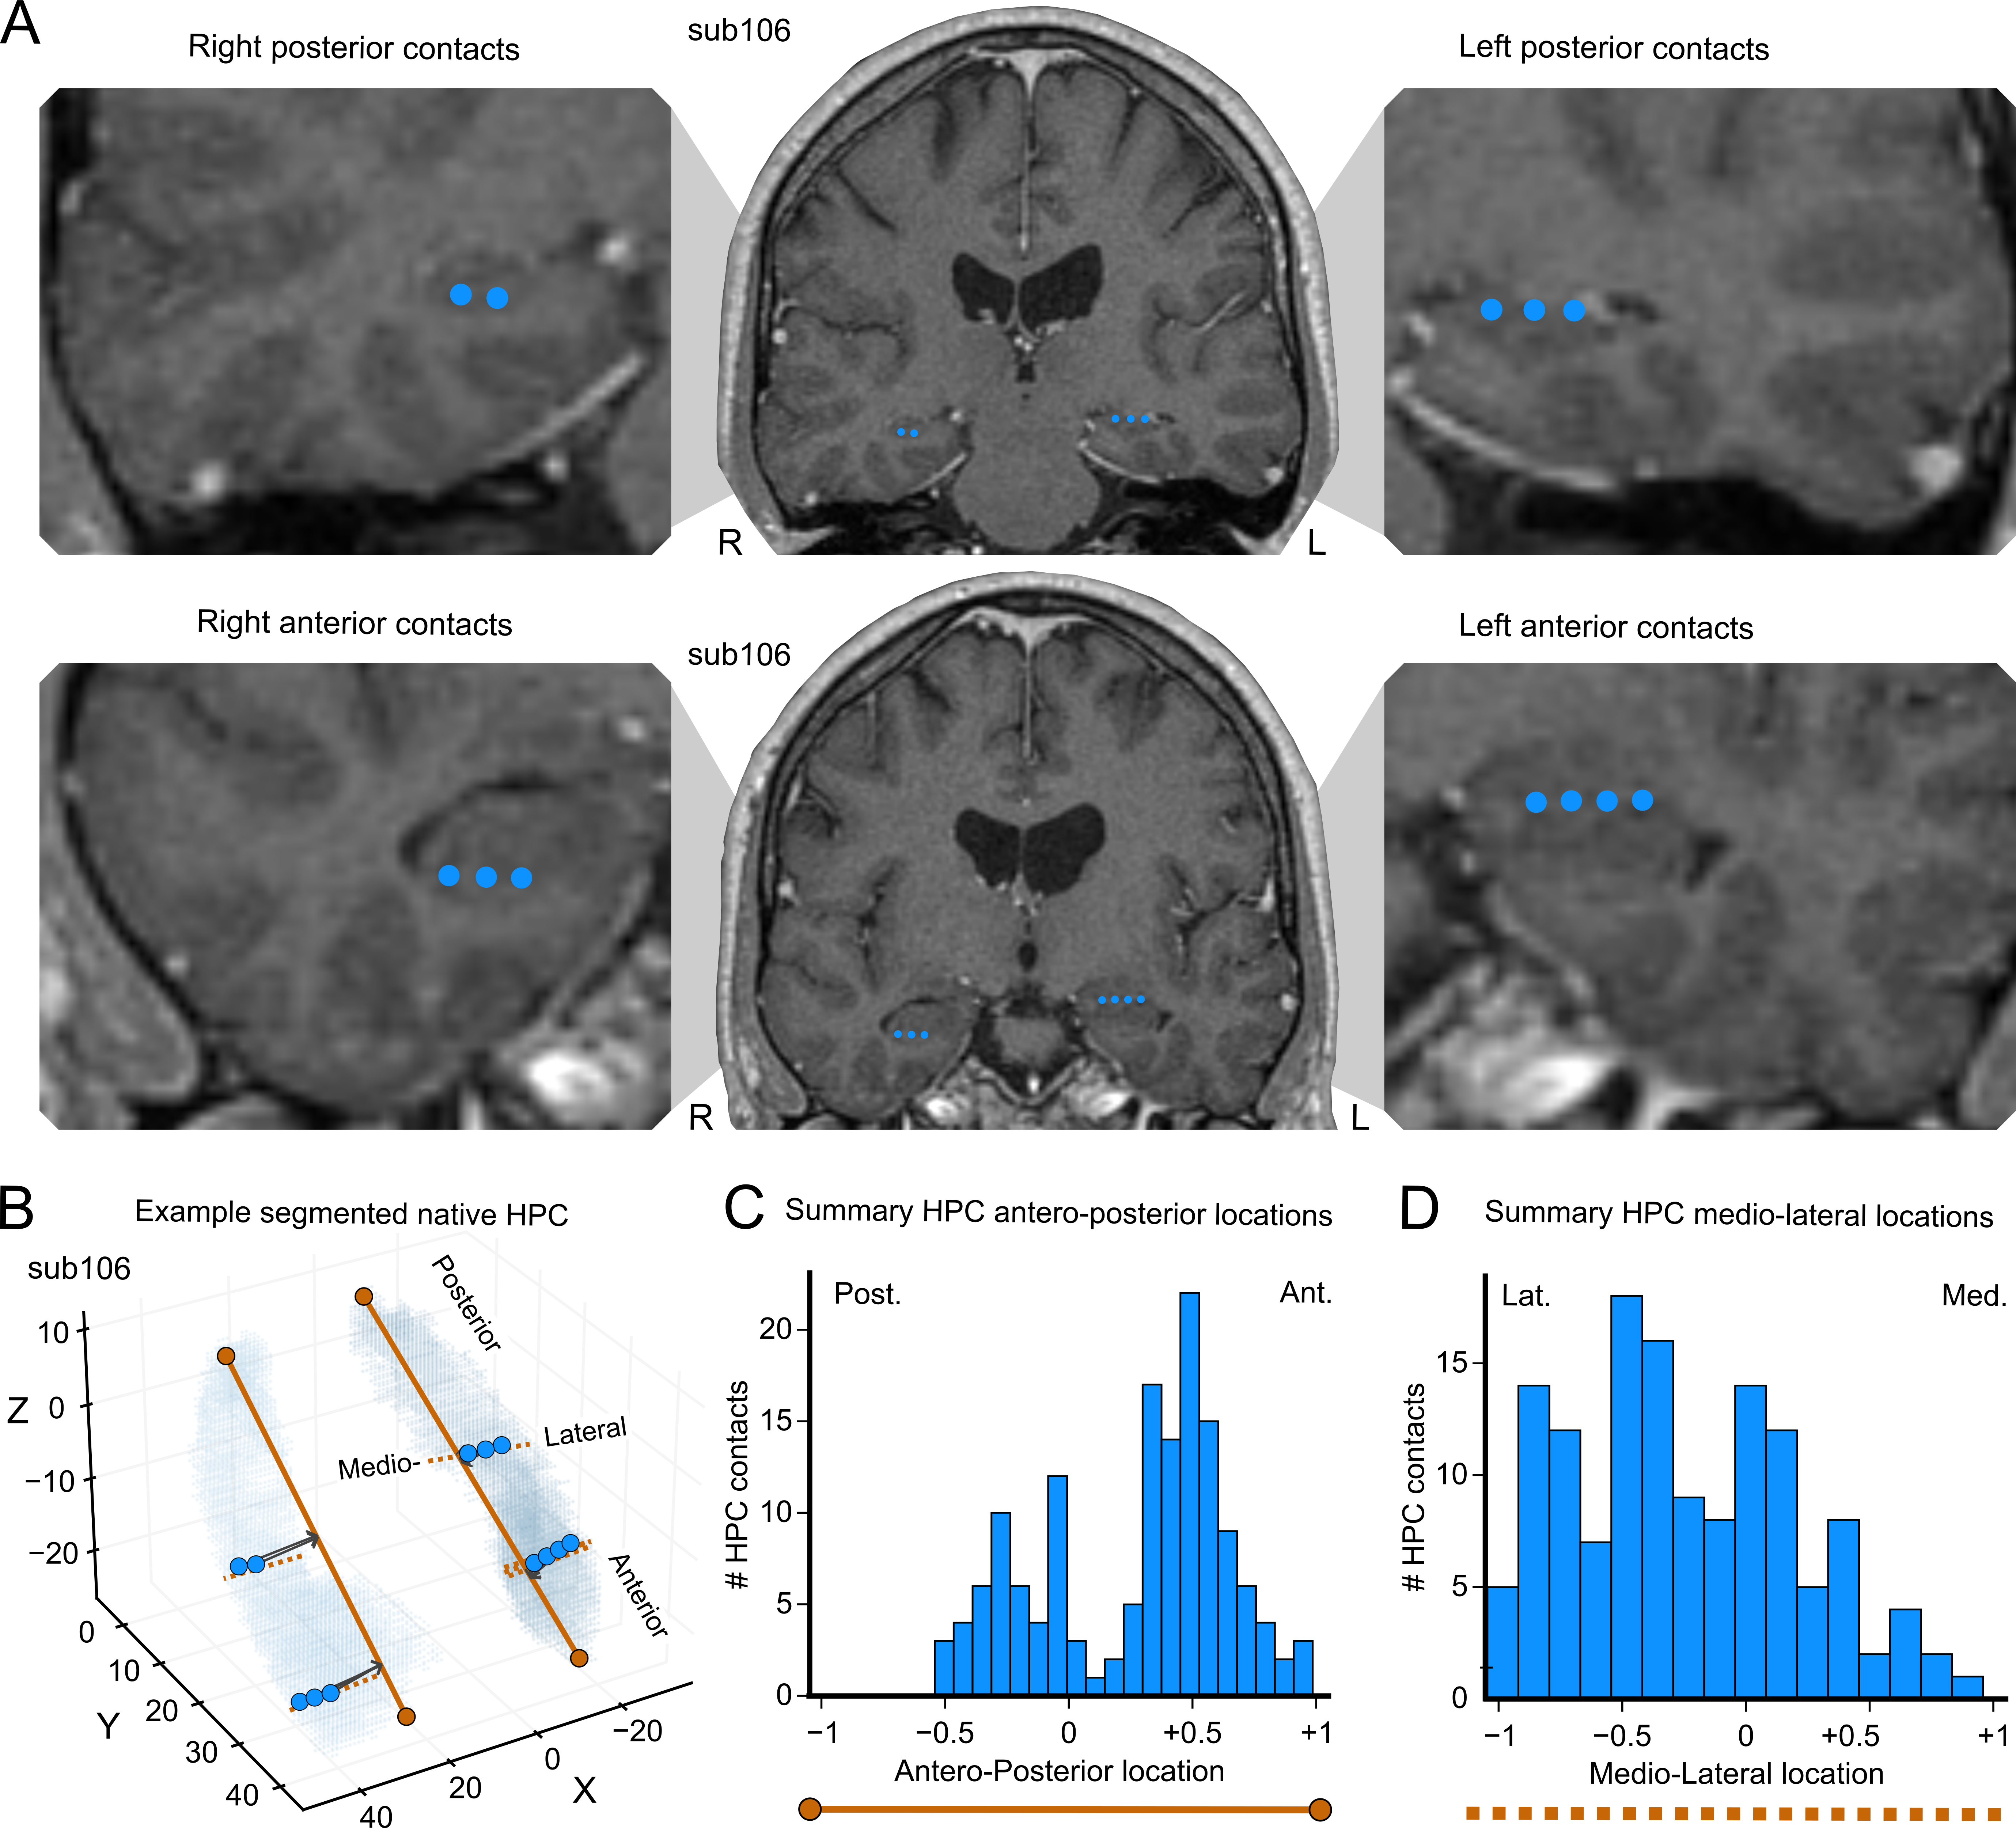
\includegraphics[width=\textwidth]{thefig_hpc-anatomy.png}
\end{center}
\captionsetup{type=figureaboveskip=6pt, belowskip=14pt}
\captionof{figure}{
    \label{fig:hpc-anatomy}
    \textbf{Anatomical localization and distribution of hippocampal electrode contacts}
    (\textbf{A}) T1-weighted MRI showing posterior (top) and anterior (bottom) hippocampal electrode contacts. Insets display higher magnifications of the right and left hemispheres.
    (\textbf{B}) 3D hippocampal volumes segmented from the same subject’s MRI with contact locations (blue dots) overlaid. Solid and dotted brown lines mark the detected antero–posterior and medio–lateral axes, respectively.
    (\textbf{C} and \textbf{D}) Distribution of hippocampal contacts along the antero–posterior (C) and medio–lateral (D) axes across all participants. Of 170 contacts, 105 were located in the right hemisphere.
}

\subsubsection{Hippocampal \gsp{lfp} are paced by a 2-Hz oscillation}
Analyzing brain oscillations often involves assuming that a given biological signal lies within a strict frequency range. This approach is efficient when this biological phenomenon is well established such as theta oscillations in mice (REF), but it constrains the analysis to prior knowledge. An alternative is to use unsupervised signal decomposition methods such as \g{emd}. \g{emd} decomposes \gp{lfp} into their constituent oscillatory components (referred to as \gp{imf}) without assuming fixed frequency bands (REF). However, several factors can influence the spectral structure of \gp{lfp} across macrocontacts and subjects. As a result, the extracted \gp{imf} may overlap in frequency (mode mixing) or may not be detected in a consistent manner across macrocontacts or participants (low consistency) (REF). These issues make it challenging to ensure that \gp{imf} are reliably identified across subjects. To address these limitations, we used a recently introduced version of masked \g{emd}, referred to as \gs{tmemd} (REF). This approach introduces controlled masking signals during decomposition to reduce mode mixing and to improve the separation of oscillatory components. In addition, mask parameters are optimized across subjects, which increases the consistency of the detected components at the group level. \gs{tmemd} therefore provides a more stable and interpretable decomposition of hippocampal \gp{lfp} than standard \g{emd}, particularly in datasets with substantial inter-individual variability. Full methodological details are provided in Appendix~\ref{apdx:acquisition}.

In participants who were awake and watching screen displays, we detected one oscillation in the human hippocampus with a peak frequency around 6 Hz (peak [80\% power band (PB)]: 6.15 [3.75 – 8.50] Hz). In addition, we identified two slower rhythms centered near 2 Hz [peak (80\% PB): 2.38 (1.25 – 3.50) Hz] and 1 Hz [peak (80\% PB): 1.08 (0.65 – 1.50) Hz] (Fig.~\ref{fig:hpc-imfs}). 

\begin{center}
    \includegraphics[width=\textwidth]{thefig_hpc-imfs.png}
\end{center}
\captionsetup{type=figure, aboveskip=6pt, belowskip=14pt}
\captionof{figure}{
    \label{fig:hpc-imfs}
    \textbf{Tailored Masked Empirical Mode Decomposition in the human hippocampus}
    (\textbf{A}) Left: Example hippocampal wide-band \gsp{lfp} traces with \gp{imf}.  
    Right: Power spectral density (PSD) of the wide-band signal (dashed line) obtained from macrocontact recording and the corresponding 1-, 2-, and 6-Hz \gp{imf}. 
    (\textbf{B}) Heatmaps showing power distributions of 1-, 2-, and 6-Hz \gp{imf} across all hippocampal contacts, illustrating that \gp{imf} were consistently detected across participants.
    (\textbf{C}) Average power spectral densities across hippocampal contacts, normalized to the maximal 2-Hz power, showing that \gp{imf} exhibited low mode mixing (thick lines indicate 80\% power bands).
}

Though we were able to detect 6-Hz oscillations in the human hippocampus, the most prominent oscillation visible in the raw \gp{lfp} traces were at 2 Hz (Fig.~\ref{fig:hpc-imfs}A). These 2-Hz oscillations were visible on both macrocontacts and tetrodes (Fig.~\ref{fig:thefig_hpc-2HzlfpSpec}). 

\begin{center}
    \includegraphics[width=\textwidth]{thefig_hpc-2HzlfpSpec.png}
\end{center}
\captionsetup{type=figure, aboveskip=6pt, belowskip=14pt}
\captionof{figure}{
    \label{fig:thefig_hpc-2HzlfpSpec}
    \textbf{Example hippocampal \gsp{lfp} showing a 2-Hz burst}
    Example 15-s hippocampal tetrode recording showing a prominent 2-Hz burst.
    From top to bottom: wide-band \gp{lfp} trace obtained from tetrode recording, \gp{imf}, and the corresponding wavelet spectrogram.
}

We confirmed this observation by applying spectral parameterization (REF; see Appendix~\ref{apdx:spectraldec}), which separates the periodic components of the \gp{psd} from the broadband, aperiodic structure of the spectrum. This procedure allowed us to quantify narrow-band oscillatory peaks independently of differences in overall spectral slope across contacts or participants. After removing the aperiodic component, the periodic residuals showed a clear prominence of the 2-Hz component in the hippocampus (Fig.~\ref{fig:hpc-power_acrossFreqs}A). Specifically, the corrected spectra yielded higher power at 2~Hz than at 1~Hz or 6~Hz (Fig.~\ref{fig:hpc-power_acrossFreqs}B), and the computed 2-Hz/6-Hz peak power ratio was consistently positive across hippocampal contacts (mean ratio [95\% \g{ci}]:  0.21 [0.15 – 0.27]; Fig.~\ref{fig:hpc-power_acrossFreqs}C). These results analysis suggest that hippocampal activity is dominated by a 2-Hz rhythm.

\begin{center}
    \includegraphics[width=\textwidth]{thefig_hpc-power_acrossFreqs.png}
\end{center}
\captionsetup{type=figure, aboveskip=6pt, belowskip=14pt}
\captionof{figure}{
    \label{fig:hpc-power_acrossFreqs}
    \textbf{2-Hz oscillations dominate in the hippocampus}
    (\textbf{A}) \gp{psd} corrected for the power law and averaged across hippocampal macrocontacts free of \gp{ied}. Shaded areas indicate mean ±~SEM. 
    (\textbf{B}) Estimation plots showing median differences between corrected 1-, 2-, and 6-Hz peak power (left), and between 2-Hz and 6-Hz peak power (right). 
    (\textbf{C}) Distribution showing positive 2-Hz/6-Hz peak power ratios in hippocampal contacts.
}

\subsubsection{Hippocampal 2-Hz oscillations are transient}
Hippocampal 2-Hz activity appeared as transient oscillatory bursts and was observable across subjects and along the hippocampal formation (Fig.~\ref{fig:hpc-2Hzbursts}).

\begin{center}
    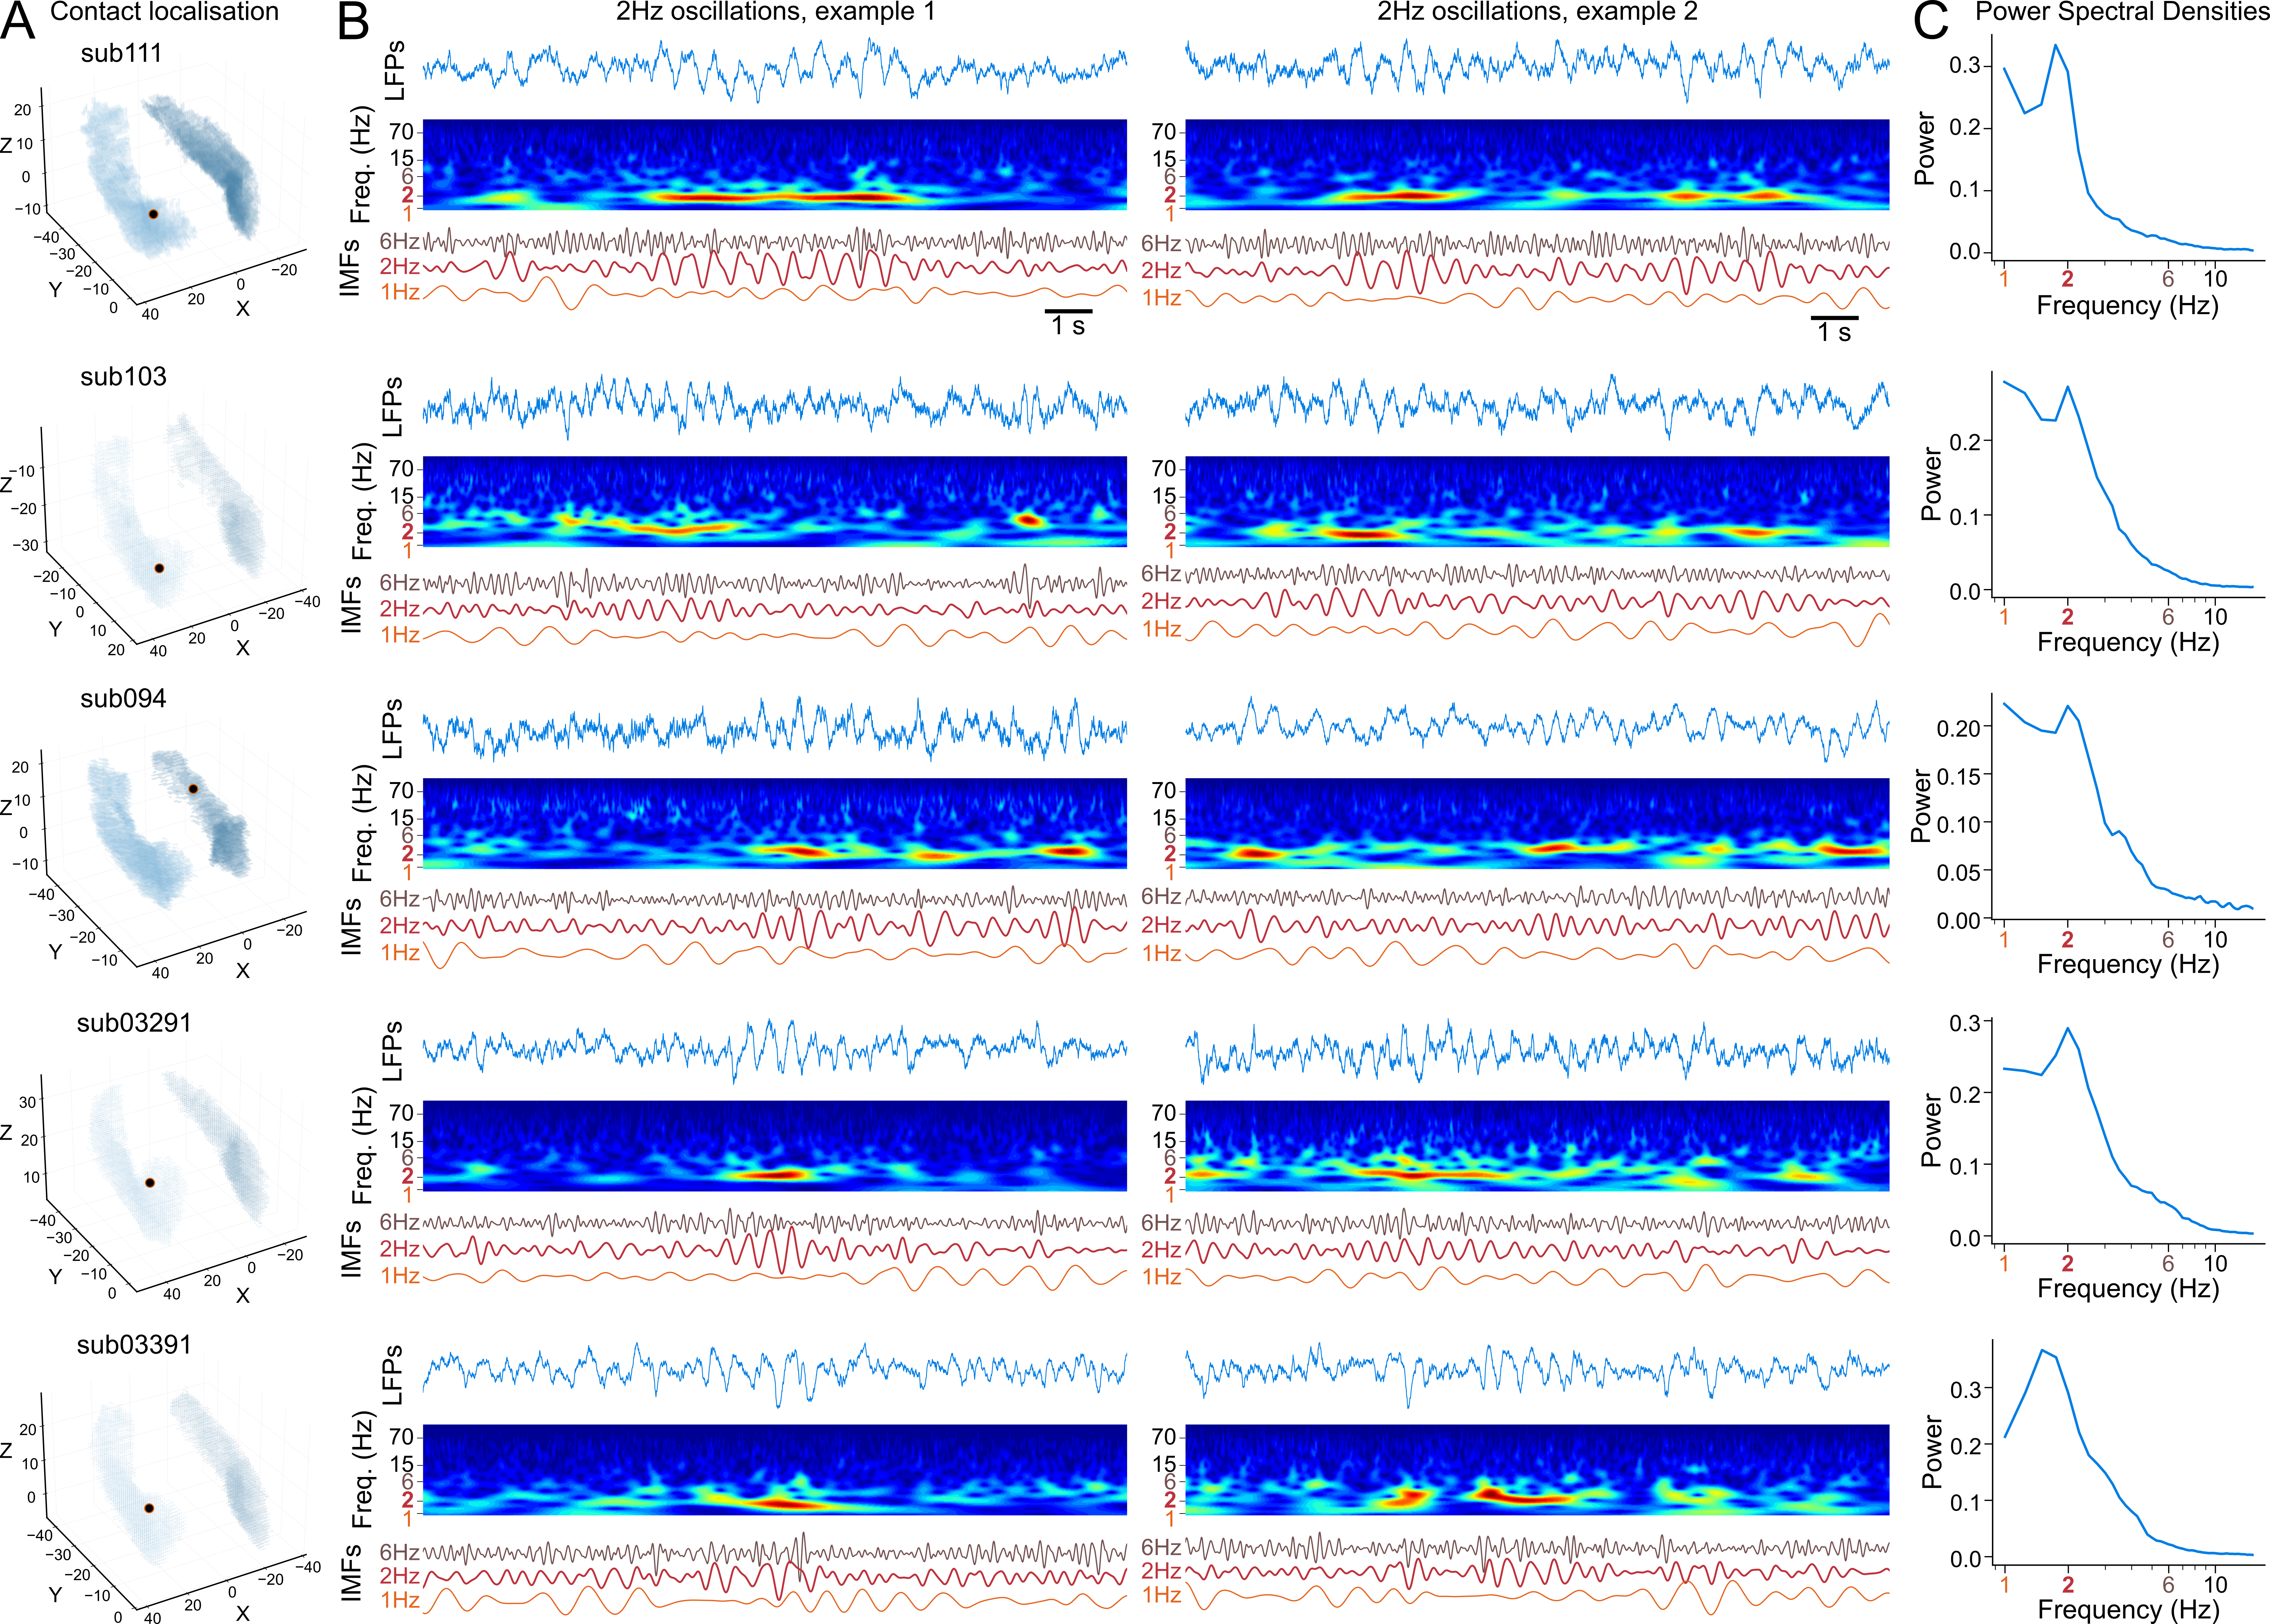
\includegraphics[width=\textwidth]{thefig_hpc-2Hzbursts.png}
\end{center}
\captionsetup{type=figure, aboveskip=6pt, belowskip=14pt}
\captionof{figure}{
    \label{fig:hpc-2Hzbursts}
    \textbf{Examples of hippocampal 2-Hz bursts}
    (\textbf{A}) 3D hippocampal volumes showing electrode contact locations used in panels B and C.
    (\textbf{B}) Example 15-s hippocampal macrocontact recordings showing 2-Hz oscillations with corresponding spectrograms and (\gp{imf}) from five participants (one row per participant).
    (\textbf{C}) \gsp{psd} averaged over the 10-min active sessions corresponding to the recordings shown in panel B. All contacts were free of \gsp{ied} (from top to bottom: 0, 0.34, 0.79, 0.33, and 0.24 discharges detected per minute).
}

To quantify these events, we used the 2-Hz \g{imf} to detect bursts defined as periods of increased power within the 1–4~Hz range, retaining only events lasting at least two oscillatory cycles (Fig.~\ref{fig:ex-burstDetection}A). For each burst, we then measured onset, offset, and duration, expressed both in seconds and in number of cycles (Fig.~\ref{fig:ex-burstDetection}B). Full methodological details are provided in Appendix~\ref{apdx:decompositions}. Across subjects, the maximal burst duration showed substantial variability (Fig.~\ref{fig:ex-burstDetection}C), consistent with the transient expression of these 2-Hz events (mean maximum number [95\% confidence interval (CI)]: 19.6 [15.8 – 23.4] cycles per burst).

\begin{center}
    \includegraphics[width=\textwidth]{thefig_ex-burstDetection.png}
\end{center}
\captionsetup{type=figure, aboveskip=6pt, belowskip=14pt}
\captionof{figure}{
    \label{fig:ex-burstDetection}
    \textbf{Detection of hippocampal 2-Hz bursts}
    (\textbf{A}) Example 27-s hippocampal \g{lfp} showing 2-Hz oscillatory bursts with corresponding spectrogram and 2-Hz \g{imf}.
    (\textbf{B}) Distributions of burst durations measured in cycles (top) and seconds (bottom) for the hippocampal macrocontact shown in panel A. A total of 174 bursts lasting at least two cycles were detected in this recall session. Arrowheads indicate the durations of the two bursts visible in panel A.
    (\textbf{C}) Distributions of maximal burst duration in cycles (top) and seconds (bottom) per recording day across participants.
}

\subsubsection{Validation of 2-Hz oscillations}

\subsubsubsection{Local referencing reduces detection of slow oscillations}
Local referencing on micro and bipolar referencing on macro
=> This is why we will be using CAR throughout the manuscript

\subsubsubsection{Slow-oscillation amplitude and \gsp{ied} rate}
Detection of IEDs (methods). IEDs are transient, non-oscillatory events. IEDs rate increases at rest. 1- and 2-Hz oscillations are more prominent in contacts clear from IEDs. 

\subsubsubsection{Phase reversal of hippocampal 2-Hz oscillations}
Echo to the introduction where we will have presented how the dipole is structured between layers, in humans and rodents. Show maybe one laminar recording from rodents. Then show phase reversal with cycle-triggered average of LFPs.

% ---------- Subsection 2: 2-Hz in memory task
\subsection{Hippocampal 2-Hz is selectively evoked in the memory task}
\subsubsection{Hippocampal 2-Hz power increase with task engagement}
Methods: one-over-f fitting. Results: Example contact; estimation plots with various controls; \gsp{lmem}. This is all using contacts free of interictal discharges (reader will understand why because we explained in the previous subsection). Burst duration is also higher in learning and recalling.

\subsubsection{Hippocampal 2-Hz bursts are evoked by mnemonic cues}
\subsubsubsection{\gsp{erp} are modulated by mnemonic engagement}
ERPs change throughout the task in the hippocampus.

\subsubsubsection{Evoked oscillations follow \gsp{erp} deflection}
Evoked 1-, 2- and 6-Hz amplitudes relate to mnemonic engagement. Correlation between evoked ERPs deflection and 2-Hz amplitude. 

\subsubsection{Hippocampal 2-Hz oscillations are not evoked by motor activity}
Methods: Stepping sessions. Results: three example contacts (PSDs) with clear 2-Hz in learning but not during stepping. Statistics on these three subjects.

Note to myself: I could as well add a small control here, using viewing and post-viewing sessions when the participants hit the space bar (second image). Paired analysis by comparing the evoked amplitude after the first (no motor activity) and the second (motor activity) image seen in a row. It may be confounded by the short term memory effect but we dont expect this to elicit a massive 2-Hz.

% --------------- Section II: 2-Hz organizes neuronal and gamma activity in the HPC
\section{Hippocampal neuronal activity is preferentially modulated at 2-Hz}

% ---------- Subsection 1: Hippocampal neurons
\subsection{Hippocampal neurons are paced at 2-Hz}
\label{subsec:2Hz-neurons}

\subsubsection{Basic firing properties of hippocampal neurons reveal 2-Hz rhythmicity}
Methods: spike sorting and quality control. Results : firing rate distributions show that slow firing neurons constituted the biggest part of our dataset. Waveform classification: mainly broad spikes. So this looks more like pyramidal neurons. Autocorrelograms at 2-Hz. Inter-spike intervals at 500 ms.

\subsubsection{Hippocampal neurons prefer 2-Hz oscillations}
Methods: \gs{ppc} and phase randomization. Results: cycle-triggered average of population rate to illustrate co-modulation at 2-Hz. Example spike-phase distribution reveals preference at 2-Hz. Quantification of spike-phase coupling using PPC.

% ---------- Subsection 2: Hippocampal gamma
\subsection{Hippocampal gamma oscillations are preferentially modulated at 2-Hz}
\subsubsection{Gamma activity correlates with spiking activity}
Methods: Detection of gamma activity (60-160 Hz). Results: Illustration of the correlation (CAR and bipolar referencing). Correlation with local VS distal gamma. 

\subsubsection{Hippocampal gamma activity is preferentially coupled to 2-Hz phase}
Methods: \gs{pac} with the modulation index and phase randomization. Results: cycle-triggered average of gamma activity to illustrate co-modulation at 2-Hz (with spikes). Example gamma-phase distribution reveals preference at 2-Hz. Quantification of phase-amplitude coupling using PAC. Control with leave one recording day out shows that the effect is not driven by one recording day. Gamma from the anterior and posterior hippocampi prefer 2-Hz (no gradient). 

\subsubsection{Holo-Hilbert amplitude modulation analysis confirms prevailing 2-Hz hippocampal modulation of gamma activity}
Methods: \gs{hhsa} with illustration. Results: 2-Hz modulation prevails in the human hippocampus. 7-Hz oscillations dominated the mouse hippocampus.

% --------------- Section III: 2-Hz organizes neuronal and gamma activity in the MTL
\section{Hippocampal 2-Hz synchronizes neuronal activity across \gs{mtl} regions}

% ---------- Subsection 1: MTL neurons
\subsection{2-Hz oscillations are preferentially observed in the \gs{mtl}}
\subsubsection{2-Hz power dominates in the \gs{mtl} and particularly in the hippocampus}
Cycle-triggered average of LFPs show that 2-Hz oscillations propagate in the MTL. PSDs across the MTL and non-MTL contacts free of IEDs. 2-Hz vs 6-Hz power ratio.

\subsubsection{Prominent 6-8Hz oscillations in the non-MTL were detected using \gs{tmemd}}
IMF PSDs in the MTL and non-MTL with example of detected 6-8-Hz bursts in the non-MTL.

\subsubsection{2-Hz oscillations are not directly evoked by mnemonic cues outside the hippocampus}
\subsubsubsection{\gsp{erp} deflections in \gs{mtl} and non-MTL regions}
ERPs become bigger with familiarity only in the hippocampus.

\subsubsubsection{\gsp{erp} deflection does not correlate with evoked 2-Hz bursts outside the hippocampus}
Measure evoked 1-, 2- and 6-Hz in other MTL and non-MTL regions. The measure of ERP deflections is adjusted to each region to match visual input. Correlation between ERP deflection and evoked 1-, 2- 6-Hz oscillations.

% ---------- Subsection 2: MTL gamma
\subsection{\gs{mtl} neurons are paced at 2-Hz}
\subsubsection{Basic firing properties of \gs{mtl} neurons reveal 2-Hz rhythmicity}
Results : Autocorrelograms at 2-Hz. Inter-spike intervals at 500 ms in the MTL. Example neuron in the non-MTL to show we can easily find 6-Hz rhythmicity in the non-MTL.

\subsubsection{\gs{mtl} neurons prefer 2-Hz oscillations in the hippocampus}
Results: cycle-triggered average of population rate in the EC and HPC to illustrate co-modulation at 2-Hz in these two example structures. Example spike-phase distribution reveals preference at 2-Hz of EC neurons. Quantification of spike-phase coupling using PPC in the MTL. \gsp{lmem} showing that MTL gamma is better modulated at 2-Hz than non-MTL gamma.

\subsection{Hippocampal 2-Hz synchronizes \gs{mtl} gamma oscillations}
Methods: distal PAC. Results: cycle-triggered average of gamma activity in the MTL. Illustration of phase-amplitude coupling across the MTL. \g{mtl} gamma activity is preferentially coupled to hippocampal 2-Hz phase = quantification of MTL preference for 2-Hz oscillations. Phase synchronization is higher during learning and recalling than viewing sessions.

Transition to Chapter 4: online => offline

% --------------------------------------------------------------------------------
% ------------------------------------ Chap 4 ------------------------------------ CHAP 4: OFFLINE
% --------------------------------------------------------------------------------
\chapter{Neural activity in the offline human hippocampus} % chap 4

% --------------- Conceptual introduction
\section{Conceptual introduction}
\subsection{The two-stage model of memory}
Online (theta) → assembly formation. Offline (ripples) → assembly reactivation.

\subsection{Hypothesis}
Human 2-Hz bursts form the online structure for memory-relevant coactivity patterns. Offline ripples should preferentially reinstate 2-Hz-structured motifs

\subsection{Analytical overview}
Ripple detection and validation, coactivity motif construction. Reactivation analysis

% --------------- Section I: Hippocampal basic physiology across sleep stages
\section{Hippocampal physiology across sleep stages}
\subsection{Hippocampal 2-Hz features \gs{rem} sleep but not \gs{sws}}
Methods: describe polysomnography. Example of 2-Hz bursts in REM. 2-Hz power across sleep stages. Maybe: propagation of 2-Hz oscillations in the rest of the MTL (hypothesis of the ponto-geniculo oscillations PGO)? 

\subsection{Hippocampal ripples feature \gs{sws} and rest sessions}
\subsubsection{Detection of hippocampal ripples}
Methods: two-step algorithm used to detect ripples. Show the templates, and the quality control used to identify reliable ripples without manual intervention.

\subsubsection{Basic properties of the ripples}
Show raw examples as well as ripple-triggered averages of LFPs and spectrograms. Distribution of ripple frequency centers around 70 Hz. Ripples ride on a sharp-wave. Ripples can be detected on the local tetrodes as well.

\subsubsection{Ripples properties across sleep stages}
Ripple rate is higher in SWS and N1 than wake and REM. Ripples detected in rest are comparable to N1. Ripples basic properties are stable between pre- and post-learning rests.

\subsubsection{Hippocampal neurons are modulated by ripples}
Trigger average (and quantification!) of the modulation of hippocampal single neurons around sharp wave ripples. Single examples and summary heatmap. 

\subsubsection{Ripples propate to the \gs{mtl}}
Ripple-triggered averages of the LFPs and ripple band in other regions (MTL and non-MTL). The propagation is more consistent in the MTL than the non-MTL. 

% --------------- Section II: Coactivity motifs in 2-Hz bursts reactivate in post-learning hippocampal ripples
\section{Neuronal coactivity motifs in 2-Hz bursts reactivate in post-learning hippocampal ripples}
\subsection{Measuring reactivation using neuronal coactivity motifs}
\subsubsection{2-Hz bursts coactivity motifs reactivate in post-learning ripples}
Methods: building coactivity matrices and measuring reactivation with MTL single-neurons. In-bursts vs out-of-bursts. 1-, 2- vs 6-Hz bursts (exclusion).

\subsubsection{Reactivtion is relevant for behavioural performance}
Learning but not viewing coactivity motifs reactivate. All controls related to learning vs viewing (firing rate, shuffled cell ID, out-of-ripples, single subjects). Best better reactivate than worst recalled associations. 

\subsection{Measuring reactivation using gamma coactivity motifs}
\subsubsection{Gamma coactivity motifs are physiologically meaningful}
 Previous figure S18: shuffling contact IDs breaks the matrices. Intra-regional coactivity is higher than inter-regional coactivity. Correlation with 2-Hz phase amplitude coupling matrices (with illustration). Idem with ripple coactivity.

\subsubsection{Gamma coactivity motifs are rigid}
All negative results on gamma coactivity, using the exact same analytical framework as with single-neurons. The aim here is to report this negative result, and echo the work done with gamma correlations in the visual field (other lab).

% --------------------------------------------------------------------------------
% --------------------------------- DISCUSSION -----------------------------------
% --------------------------------------------------------------------------------
\chapter{Discussion}

Limits: what happens out of the oscillatory bursts? Noise does not exist in physiology: what information do these out-of-bursts epochs carry? These would be epochs where the firing rate is higher (aperiodic components), fractal measures are higher, but it remains unclear what is actually happening there for the network. Is it really "not" communicating with other structures? If yes, how does it communicate? What are the alternatives mechanisms to "communication through coherence"? Main challenge to study this is that the rodent hippocampus is virtually always paced by theta. Then maybe that would be the biggest inter-species difference we find: transient oscillations. Note: it could be useful to illustrate this discussion to show 6-8Hz in the temporal cortex as well.

% --------------------------------------------------------------------------------
% ---------------------------- METHODS APPENDICES --------------------------------
% --------------------------------------------------------------------------------

\appendix

% --------------- Appendix A: Data acquisition 
\chapter{Appendix: Neurophysiological recordings and analysis of oscillations}

\section{Data acquisition and preprocessing}
\label{apdx:acquisition}
\subsection{Participants}
\subsection{Electrode models}
\subsection{Co-registration and anatomical verification}
\subsection{Neurophysiological recordings}
\subsection{Detection of \gsp{ied}}

\section{Decomposing \gsp{lfp} into oscillatory components}
\label{apdx:decompositions}
\subsection{Rationale for IMF-based decomposition}
Here we will describe the optimization steps, final parameters of the masks used. Also Examplify non-linearity of the signal (phase-frequency plots)
\subsection{Mask optimization and criteria}
\subsection{Cycle detection and quality control}
\subsection{Detection of oscillatory bursts}

\section{Other spectral decompositions}
\label{apdx:spectraldec}
\subsection{\gsp{psd} estimation (Welch)}
\subsection{Aperiodic correction using spectral parameterization}
\subsection{Morlet wavelet spectrogram parameters}
\subsection{Stimulus-locked spectral amplitude estimation}
\subsection{Detection of gamma activity}

\section{Cross-frequency analyses}
\subsection{\gs{pac} and phase randomization}
\subsection{\gs{hhsa}}

% --------------- Appendix B: Single-neuron analyses
\chapter{Appendix: Analysis of single-neuron activity}

\section{Spike sorting and single-unit validation}
\subsection{Automated pipeline}
\subsection{Manual curation quality criteria}
\subsection{Waveform classification}

\section{Spike-field relationship}
\subsection{\gs{ppc} and phase randomization}
\subsection{Spike-gamma relationship}

% --------------- Appendix C: Hippocampal ripples and reactivation
\chapter{Appendix: Hippocampal ripples and reactivation}

\section{Ripple detection and validation}
\subsection{Initial ripple detection}
\subsection{Template matching}
\subsection{Final detection and quality controls}
\subsection{Ripple-triggered averages}
\subsection{Characterization of ripple central frequency}

\section{Detection of cross-regional coactivity motifs}
\subsection{Epochs selection}
\subsection{Using single-neurons}
\subsection{Using gamma activity}

\section{Reactivation of coactivity motifs in hippocampal ripples}
\subsection{\gsp{glm}}
\subsection{Controls}

% --------------- Appendix D: Statistical analyses
\chapter{Appendix: Statistical analyses}
\section{Bootstrap and permutation tests}
\section{\gsp{glm} and \gsp{lmem}}
\section{Cluster-based permutation}

\end{document}